\documentclass[fleqn]{jbook}
\usepackage{physpub}

\begin{document}

\begin{question}{専攻 問題1}{}

% Definition of local macros

\parbox[t]{100mm}{
質量$m$の粒子が半径$a$深さ$V_{0}$の井戸型ポテンシャル
%
\[ V(r)= \left\{ \begin{array}{lc}%
         -V_{0} & (r \leq a) \\
             0  & (r>a)      \end{array} \right. \]
%
の中を運動する。次の設問に答えよ。
%
}\parbox[t]{60mm}{\vspace*{-8mm}
\begin{center}
  \mbox{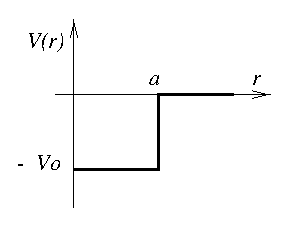
\includegraphics[clip]{1995phy1-1.eps}}
\end{center}}
%

\begin{subquestions}
\SubQuestion

  波動関数を極座標$(r,\theta,\phi)$で
  \[ \Psi (r ,\theta ,\phi )=R_{\ell}(r)Y_{\ell m}(\theta,\phi) \]
  のように表したとき$R_{\ell}(r)$が従う方程式を書け。ただし、
  ラプラシアンを極座標で書くと
%
  \[ \Laplacian = \frac{1}{r^2} \Partial{}{r}r^2 \Partial{}{r}%
                + \frac{\Operator{\Lambda}}{r^2}  \hspace{15mm}%
     \Operator{\Lambda} = \frac{1}{\sin \theta} \Partial{}{\theta} \sin\theta \Partial{}{\theta}%
                + \frac{1}{\sin^2\theta}\Partial{^2}{\phi^{2}} \]
%
  のように表される。また、$Y_{\ell m}(\theta,\phi)$は球面調和関数で
  演算子$\Operator{\Lambda}$の固有関数である。
%
  \[ \Operator{\Lambda} Y_{\ell m}(\theta,\phi) = -\ell(\ell+1)Y_{\ell m}(\theta,\phi) \]
%
  \SubSubQuestion
    $V_{0}$のある値についてはs状態$(\ell=0)$に束縛状態が一つだけあり、
    その束縛エネルギー$\varepsilon$は$V_{0}$に比べて十分小さい
    $(0<\varepsilon \ll V_0)$。

  \begin{subsubquestions}
  \SubSubQuestion
    ポテンシャルの深さ$V_{0}$を求めよ。

  \SubSubQuestion
    上の束縛状態での井戸の外$(r>a)$に粒子が存在する確率を計算せよ。

  \end{subsubquestions}


\SubQuestion
  次に同じポテンシャルによる散乱を考える。各$\ell$で$r$の十分大きい
  ところで
%
  \[ R_{\ell}(r) \sim A_{\ell} \frac{ \sin{(kr- \frac{1}{2}\ell \pi + \delta_{\ell})}}{r} \]
%
  で表されているとき、$\delta_{\ell}$ を位相のずれという。(ii)と同じ
  $V_{0}$の値について入射エネルギーが$E=\frac{9V_{0}}{16}$のとき、
  s波($\ell=0$)の位相のずれの正接$ \tan \delta_{0}$を求めよ。

\end{subquestions}
\end{question}
\begin{answer}{専攻 問題1}{}
 \begin{subanswers}
  \SubAnswer
Schr\"odinger方程式
  \[
  \biggl(-\frac{\hbar^2}{2m}\Delta+V\biggr)\Psi=E\Psi
  \]
で、ラプラシアンを極座標で表し、波動関数の動径部分$R_l$が満すべき方程式を
抽出すると、以下の通りとなる。
  \begin{equation}
   \biggl(\frac{1}{r^2}\Deriver{}{r}r^2\Deriver{}{r}-\frac{l(l+1)}{r^2}\biggr)R_l
    =-\frac{2m}{\hbar^2}(E-V)R_l
  \end{equation}
  \SubAnswer
  \begin{subsubanswers}
   \SubSubAnswer
   s状態を考えるので$l=0$であり、また、
   $\frac{1}{r^2}\Deriver{}{r}r^2\Deriver{}{r}=\frac{1}{r}\Deriver{^2}{r^2}r$
   に注意すると、$R_0$が満す方程式は、
   \begin{align}
    \begin{array}{ll}
     \displaystyle{\Deriver{^2}{r^2}(rR_0)=
      -\frac{2m}{\hbar^2}(V_0-\varepsilon)(rR_0)}
      & \mbox{(井戸の中)} \\
     \displaystyle{\Deriver{^2}{r^2}(rR_0)=
      \frac{2m}{\hbar^2}\varepsilon(rR_0)}
      & \mbox{(井戸の外)}
    \end{array}  
   \end{align}
   これより、$R_0$は、全体を定数倍する任意性を除けば、
   \begin{equation}
    R_0=
     \begin{cases}
      \displaystyle{\frac{1}{r}
      \sin\biggl(\frac{\sqrt{2m(V_0-\varepsilon)}}{\hbar}r+\delta\biggr)}
      & (r<a) \\
      \displaystyle{
      \frac{C_1}{r}\exp\biggl(-\frac{\sqrt{2m\varepsilon}}{\hbar}r\biggr)
      +\frac{C_2}{r}\exp\biggl(\frac{\sqrt{2m\varepsilon}}{\hbar}r\biggr)}
      & (r>a)
     \end{cases}
     \eqname{eq:ro1}
   \end{equation}
   ($C_1,C_2,\delta$は定数)と書ける。

   ここで、波動関数の規格化可能性より、$C_2=0$。また原点で、ポテンシャルが
   特異性を持たないことより、$\delta=0$と決まる。

   残った定数$C_1$は、$r=a$で\eqhref{eq:ro1}の第1、第2式が滑らかにつながるよ
   うに決定される。この条件は、
   \begin{equation}
    \begin{cases}
     \displaystyle{
     \frac{1}{a}\sin\biggl(\frac{\sqrt{2m(V_0-\varepsilon)}}{\hbar}a\biggr)
     =\frac{C_1}{a}\exp\biggl(-\frac{\sqrt{2m\varepsilon}}{\hbar}a\biggr)} \\
     \displaystyle{
     \frac{\sqrt{2m(V_0-\epsilon)}}{\hbar}
     \cot\biggl(\frac{\sqrt{2m(V_0-\varepsilon)}}{\hbar}a\biggr)
     =-\frac{\sqrt{2m\varepsilon}}{\hbar}}
    \end{cases}
    \eqname{eq:cond1}
   \end{equation}
   $0<\varepsilon\ll V_0$より、$\varepsilon/V_0=0$としてよい。すると、
   \eqhref{eq:cond1}第2式より、
   \begin{align*}
    & \cot\biggl(\frac{\sqrt{2mV_0}}{\hbar}a\biggr)
    =-\sqrt{\frac{\varepsilon}{V_0}}=0 \\
    & \Longrightarrow\frac{\sqrt{2mV_0}}{\hbar}a
    =\biggl(n+\frac{1}{2}\biggr)\pi\qquad(n=0,1,2,\cdots)
   \end{align*}
   s状態に束縛状態がただ一つあるということは、その束縛状態の固有関数が
   $r<a$に節を持たないことを意味する。即ち、$n=0$である。
   \begin{align*}
    \therefore\quad V_0 &= \biggl(\frac{\pi}{2}\biggr)^2
    \biggl(\frac{\hbar}{a}\biggr)^2\bigg/2m \\
    &= \frac{\pi^2\hbar^2}{8ma^2}
   \end{align*}
   \SubSubAnswer
   このとき、\eqhref{eq:cond1}第1式は、
   \[
   \sin\biggl(\frac{\pi}{2}\biggr)
   =C_1\exp\biggl(-\frac{\sqrt{2m\varepsilon}}{\hbar}a\biggr)
   \]
   となり、
   \[
   C_1=\exp\biggl(\frac{\sqrt{2m\varepsilon}}{\hbar}a\biggr)
   \]
   よって、求める確率は、
   \begin{align*}
    \frac{\int_{a\leq r<+\infty}|\Psi|^2d^3r}
    {\int_{0\leq r<+\infty}|\Psi|^2d^3r}
    &= \frac{\int d\Omega|Y_{00}|^2\int_a^{+\infty}dr\cdot r^2|R_0|^2}
    {\int d\Omega|Y_{00}|^2\int_0^{+\infty}dr\cdot r^2|R_0|^2} \\
    &= \frac{\int_a^{+\infty}dr
    \exp\bigl(2\frac{\sqrt{2m\varepsilon}}{\hbar}a\bigr)
    \exp\bigl(-2\frac{\sqrt{2m\varepsilon}}{\hbar}r\bigr)}
    {\int_0^adr\sin^2\bigl(\frac{\pi}{2}\frac{r}{a}\bigr)
    +\int_a^{+\infty}dr
    \exp\bigl(2\frac{\sqrt{2m\varepsilon}}{\hbar}a\bigr)
    \exp\bigl(-2\frac{\sqrt{2m\varepsilon}}{\hbar}r\bigr)} \\
    &= \frac{\frac{\hbar}{2\sqrt{2m\varepsilon}}}
    {\frac{a}{2}+\frac{\hbar}{2\sqrt{2m\varepsilon}}} \\
    &= \frac{1}{1+\frac{\sqrt{2m\varepsilon}}{\hbar}a}
   \end{align*} 
  \end{subsubanswers} 
  \SubAnswer
  $(\sqrt{2mV_0}/\hbar)a=\pi/2$であること、及び、井戸の内では
  $E-V=(25/16)V_0$、井戸の外では$E-V=(9/16)V_0$であることに注意すると、
  $R_0$が従う方程式は、
  \begin{equation}
   \Deriver{^2}{r^2}(rR_0)=
    \begin{cases}
     \displaystyle{-\biggl(\frac{5\pi}{8}\biggr)^2\frac{1}{a^2}(rR_0)}
     & \mbox{(井戸の中)} \\
     \displaystyle{-\biggl(\frac{3\pi}{8}\biggr)^2\frac{1}{a^2}(rR_0)}
     & \mbox{(井戸の外)}
    \end{cases}
  \end{equation}
  \textbf{2(i)}と同様の考察により、$R_0$は、
  \begin{equation}
   R_0=
    \begin{cases}
     \displaystyle{\frac{1}{r}\sin\biggl(\frac{5\pi}{8}\frac{r}{a}\biggr)}
     & (r<a) \\
     \displaystyle{\frac{C}{r}\sin\biggl(\frac{3\pi}{8}\frac{r}{a}
     +\delta_0\biggr)} & (r>a)
    \end{cases}
  \end{equation}
  ($C$は定数)と書ける。これらが、$r=a$で滑らかにつながることより、$rR_0$の
  対数微分が$r=a$で一致する。よって、
  \begin{align}
   & \frac{5\pi}{8}\cot\biggl(\frac{5\pi}{8}\biggr) 
   = \frac{3\pi}{8}\cot\biggl(\frac{3\pi}{8}+\delta_0\biggr)\notag\\
   & \Longleftrightarrow
   \tan\biggl(\frac{3\pi}{8}+\delta_0\biggr)
   =\frac{3}{5}\tan\biggl(\frac{5\pi}{8}\biggr) \notag\\
   & \mspace{-18.0mu}\mbox{加法定理を用いて、左辺の$\tan$を分解して整理
   すると} \notag\\
   & \Longleftrightarrow
   \tan\delta_0=\frac{\frac{3}{5}\tan\frac{5\pi}{8}-\tan\frac{3\pi}{8}}
   {1+\frac{3}{5}\tan\frac{3\pi}{8}\tan\frac{5\pi}{8}}\eqname{eq:delta0}
  \end{align}
  一方
  \[
   \tan\frac{5\pi}{8}=\tan\biggl(\pi-\frac{3\pi}{8}\biggr)=-\tan\frac{3\pi}{8}
  \]
  及び、$\tan$の加法定理
  \begin{align*}
   1 &= \tan\biggl(\frac{5\pi}{8}-\frac{3\pi}{8}\biggr) \\
   &= \frac{\tan\frac{5\pi}{8}-\tan\frac{3\pi}{8}}
   {1+\tan\frac{5\pi}{8}\tan\frac{3\pi}{8}}
  \end{align*}
  より、
  \[
  \tan\frac{3\pi}{8}=1+\sqrt{2},\qquad\tan\frac{5\pi}{8}=-1-\sqrt{2}
  \]
  なので、これを\eqhref{eq:delta0}に代入して計算すると、
  \[
   \tan\delta_0=\frac{8+2\sqrt{2}}{7}
  \]
  となる。
 \end{subanswers}
\end{answer}

\end{document}
